\section{\textcolor[HTML]{D32F2F}{Kravspesifikasjon}}

\subsection{Tjenestedesign}


Tjenesteservice vs produktservice\\
Styrke vs nytte vs service


\subsubsection{Segmentering og målgrupper}
Et segment betyr \textit{del av noe}, og innebærer å dele opp et marked i flere interesseområder. Målgrupper relaterer seg som grupper av personer med fellestrekk innenfor kjønn, alder, interesser, bosted, utdanning eller lignende.(Kilde snl) Ved å velge en spisset målgruppene og se den i sammenheng med et segment kan man drive mer målrettet og treffsikker markedsføring, eller konseptutvikling i dette tilfellet. (Kilde ndla) 
\\\\
Gruppen besøkte Sirkus shopping og gjorde observasjon av handlemønster blant personer inne på senteret. Ut fra dette feltstudiet fikk gruppen en god oversikt og kunne foreta en segmentering av handlemønster og analysere hvilke målgrupper som befant seg på senteret. 
Gjennom feltstudiet knyttet gruppen målgruppene opp mot segmenteringen, se Tabell \ref{tab:segmenterogmålgrupper}, og valgte travle mødre og fedre som segment og målgrupper. Grunnen til denne beslutningen var fordi det var disse som var mest framtredende under observasjonen og noe gruppen syntes var interessant å utforske videre.

\begin{table}[H]
    \caption{Segmenter og målgrupper}
    \label{tab:segmenterogmålgrupper}   
    \centering
    \begin{tabular}{|L{5em} L{15em} L{22em}|}
    \hline
        \rowcolor[HTML]{D32F2F}
        \textbf{\textcolor{white}{Segmenter}} & \textbf{\textcolor{white}{Målgrupper}} &
        \textbf{\textcolor{white}{Beskrivelse}}\\
        \rowcolor[HTML]{E6E6E6}
        Travle & Mødre, fedre, menn, forretningspersoner & Målrettede handlere som er raske mellom butikker \\
        Fingåere & Mødre, unge/ungdommer, Kvinner, Eldre & Noen har et mål andre ikke. Går rolig gjennom senteret, uten å stresse \\
        \rowcolor[HTML]{E6E6E6}
        Hengere & Unge/ungdommer & Ingen mål. Er på senteret for det sosiale \\
        Sittere & Unge/ungdommer, menn, fedre, eldre, mødre & Ønsker å møte folk, eller er med andre på handletur\\
        \hline
    \end{tabular}
\end{table}
%(BEDRE FOR FOR DISSE SEGMENTENE??? HAHAH)

\subsubsection{Personas}
Personas er oppdiktede karakterer som skal representere en målgruppe og et markedssegment\cite{feltstudie}. Oppgaven til en personas er å representere målet og oppførselen til den spesifikke målgruppen. Dette er nyttig når det kommer til avgjørelser angående design, interaksjon og egenskapene til produktet. Ved å gi denne målgruppen et ansikt, vil det hjelpe utviklerne av produktet med å relatere seg mer brukerne, og få mer empati. %(NOEN KILDER MÅ INN HER...kan sikkert refere til preece?)
\\\\
Gruppen valgte å fokusere på travle småbarnsforeldre, ut fra resultater gjort etter segmentering og målgruppeanalyse i Tabell \ref{tab:segmenterogmålgrupper}. På bakgrunn av dette endte vi opp med Roar og Trude som skal representere travle foreldre av begge kjønn, med barn i forskjellige alder. Disse personasene lagde vi med programmet Xtensio, der vi bestemte personlighet, mål, frustrasjoner og motivasjon som var typisk for denne brukergruppen.

%sett inn roar her
%sett inn trude her

\noindent\textbf{Scenario: Trude på handletur}\\
Trude er en 33 år gammel dame som jobber som lærer. Hun har to barn, Tina og Thomas, og er gift med Trond. På fritiden liker Trude å gå tur i skog og mark, bake og sy. Hun jobber som klasseforstander for en 4. klasse ved Strinda barneskole, og trives godt i jobben sin. Sønnen til Trude, Thomas, trenger nye fotballsko, pluss at Tina skal i fødselsdag på lørdag og må finne en presang hun kan gi venninnen. Trude tar dermed med seg begge barna på Sirkus shopping slik at de kan få ordnet begge deler samtidig. 
\\\\
Når de kommer fram på Sirkus shopping parkerer Trude bilen i parkeringshuset og leier ungene inn på senteret. Tina vil veldig gjerne inn i lekebutikken for å se på dukkene, men Trude må si nei og si at de først skal finne fotballsko til Thomas. De går inn på MX Sport og får hjelp av en av de ansatte. Tina synes det er ganske kjedelig å se på storebroren prøve sko, og begynner å gå rundt i butikken for å se om hun finner noe hun kan leke med. Trude kan ikke underholde begge to samtidig og tenker det går fint om Tina får bort og ser på de rosa jentesyklene borte i hjørnet. Thomas bestemmer seg til slutt for et par røde fotballsko med svarte striper. Trude betaler i kassen og Tina kommer etter. Hun forteller moren at hun må tisse, og de må dermed finne det nærmeste toalettet. Thomas får i oppgave å bære posen med fotballskoene, og kan vente i Fotballbutikken mens Tina og Trude går på toalettet.

\noindent\textbf{Scenario: Roar er alene hjemme}\\
Roar er en 45 år gammel mann som jobber som ingeniør. Han bor i Trondheim, og er gift med Ingunn. Hun jobber som flyvertinne. Sammen har de to barn, Ingrid og Martin. På fritiden liker Martin å gå tur i skog og mark, men får ikke så mye tid til dette fordi Ingunn ofte er bortreist i jobbsammenheng og begge barna er i tenårene. De krever tett oppfølging, og Roar bruker mye tid på leksehjelp, kjøring av barna og husarbeid. 
\\\\
Ingrid fyller snart år, og Ingunn har planlagt bursdagsfest for datteren. Hun skal feire hjemme, og Ingunn har satt opp en handleliste. Selskapet skal være lørdag kveld, og Ingunn hadde planlagt å handle torsdag kveld. Onsdag formiddag får hun en telefon fra jobben med spørsmål om hun kan ta en ekstra vakt siden en av kollegene har blitt syke. Ingunn sier ja, og ber Roar ta ansvar for å handle inn til fødselsdagen. Han er ikke så veldig komfortabel med å reise på Sirkus shopping. Han synes det er litt uoversiktlig med mange butikker, og det er tross alt Ingunn som pleier å handle. Han vet heller ikke helt hva Ingrid har lyst til å ha på festen sin, siden kona kun har skrevet ting som “brus” og “kake” og ikke spesifisert helt hva han skal kjøpe.

\subsubsection{Spørreundersøkelse}
Spørreundersøkelser er en veletablert teknikk for å samle demografisk data og meninger fra brukere\cite[s.~244]{preece}. Spørreundersøkelsene kan ha åpne eller lukkede spørsmål, avhengig av hva man ønsker å finne ut. Det viktige når man gjør spørreundersøkelser er å stille de riktige spørsmålene. De skal ikke lede brukeren på vei, slik at de svarer det man ønsker å høre. Spørsmålene som stilles må være nøytrale, og la brukeren selv gjøre seg opp en mening om temaet.
Spørreundersøkelser kan struktureres på mange måter. Noen spørsmål kan være åpne, for eksempel med tekstfelt hvor brukeren kan skrive inn sitt eget svar. Andre spørsmål kan bestå av svaralternativer, det brukeren skal velge ett eller flere alternativ som de mener er best. Et eksempel kan være på demografiske spørsmål\cite[s.~245]{preece}. Brukeren kan velge kjønn, blant to alternativer (mann, kvinne). Det kan også spørres om alder, hvor brukeren skal velge ett alternativ blant flere; 10-15, 16-20, 21-25, 26-30 osv. Man kan også lage skalaer hvor brukeren kan rangere svaret sitt. Her er det vanlig å enten bruke tallene en til fem, eller sterkt enig til sterkt uenig.
\\\\
Undersøkelsen gruppen lagde hadde fokus på å finne ut demografi og behov til brukerne av kjøpesentre, og da spesielt Sirkus shopping. Spørreundersøkelsen ble laget i Google Forms, som er en gratis digital tjeneste for spørreskjemaer. Her legger man inn spørsmål, og kan velge mellom flere svarformer som feks. ett svar, flere svar eller åpne tekstfelt. Undersøkelsen deles med en link til brukerne, og svarene kan så enten vises grafisk med diagrammer eller som rådata i Microsoft Excel regneark. Dette gjorde det svært enkelt for gruppen å dele undersøkelsen og analysere resultatene i ettertid. Resultatene fra spørreundersøkelsen, med spørsmålene som ble stilt, er vedlagt i Appendix \ref{App:AppendixA}.
\\\\
Det gruppen kunne se ut fra de 51 svarene som de fikk på spørreskjemaet var i hovedsak at de aller fleste (98\%) hadde smarttelefon (se Figur \ref{fig:smarttelefon}), og dersom dette gjenspeiler kjøpesenterets brukergruppe ellers så vil de aller fleste kundene kunne ta i bruk en app. 41,5 prosent av brukerne svarte at de var på shopping 2-4 ganger i måneden (se Figur \ref{fig:shopping}), mens 25,5 prosent svarte de var på shopping kun én gang i måneden. Nesten sytti prosent av brukerne svarte at de har et spesifikt mål med handleturen (se Figur \ref{fig:formal}), mens litt under femti prosent svarer at de går i butikkene for å titte. En gjenganger blant svarene på hva som irriterer brukerne når de oppholder seg på senteret er at det er for mye mennesker (54,9\%), at de ikke finner ønsket produkt (56,9\%) og at senteret er uoversiktlig (37,3\%) (se Figur \ref{fig:irritasjonsmoment}). Nesten 61 prosent av de spurte har aldri brukt en app for å forbedre handleopplevelsen, mens noen nevner apper som Mattilbud, Prisjakt og Zalando. Videre svarer 72,5 prosent at de gjerne hadde brukt en slik app dersom det fantes (se Figur \ref{fig:brukeapp}), og det tolket gruppen som at brukerne var positive til at det ble utviklet en app for formålet. til slutt ble det spurt om brukerne hadde et forslag til hva en slik app kunne inneholde. Da kom det forslag om blant annet lagerbeholdning, pris på varer, butikkoversikt, tilbud, rabatter og strekkodescanner.
\\\\
Det må nevnes at spørreundersøkelsen antakeligvis ikke har et representativt utvalg. Undersøkelsen ble sendt på nett, og distribuert i nettverket til de fire gruppemedlemmene. Det betyr at man ikke har nådd de som for eksempel ikke har Internett tilgjengelig, eller at man har kun nådd spesielle grupper fordi gruppen ikke har bredt nok nettverk. Antall svar på undersøkelsen er også forholdsvis få, men gruppen valgte likevel å bruke resultatene de fikk. 
\\\\
%flytte til et annet sted!
Intervjuer kan sies å være en samtale med en mening\cite{kahn}. Hvordan et intervju gjøres avhenger av intervjueren. Noen intervju kan flyte som en vanlig samtale, mens andre intervju kan være styrt av forhåndsbestemte spørsmål. Man kan si at det finnes fire hovedtyper av intervjuer: ustrukturerte, strukturerte, semi-strukturerte og gruppeintervjuer \cite[s.~233]{preece}. De første tre beskriver hvor mye intervjueren styrer samtalen, mens den siste beskriver en gruppe som ledes av en intervjuer. 

\subsubsection{Kundereiser}
\label{sec:kundereise}
Kundereiser er grafiske framvisninger med utgangspunkt i ulike synspunkt av hvordan et system oppfører seg i en gitt prosess\cite{servicedesign}. De ulike synspunktene/perspektivene blir sett på så ulike kunder av systemet, med ulike formål. I en slik framvisning blir en prosess, \textit{lifecycle stages}, identifiseres kundens berøringspunkter, \textit{touchpoints}, mot systemet, samt kundes tanker og overordnede opplevelse gjennom hele prosessen. Ved å lage kundereiser får man større forståelse for de ulike kundenes behov og kan gjøre det enklere å definere funksjoner som systemet må inneholde\cite{servicedesign}.
\\\\
I prosjektet identifiserte gruppen tre ulike kunder, med interesse i og bruk for i applikasjonen. Kunden på senteret, den ansatte i de 128 butikkene og den ansatte på lageravdelingen på Sirkus shopping. For å presentere dem valgte gruppen å ha en statisk livssyklus blant alle kundene, da alle tilknyttes samme prosess gjennom bruke av applikasjonen. Derimot ble berøringspunktene, tankene og humøret forskjellig, da de har ulike roller og oppgaver i en handleprosess. I Figur \ref{fig:customerKunde}, Figur \ref{fig:customerAnsatt}, Figur  \ref{fig:customerLager}, vises hver av disse perspektivene presentert som en kundereise. 

\begin{figure}[H]
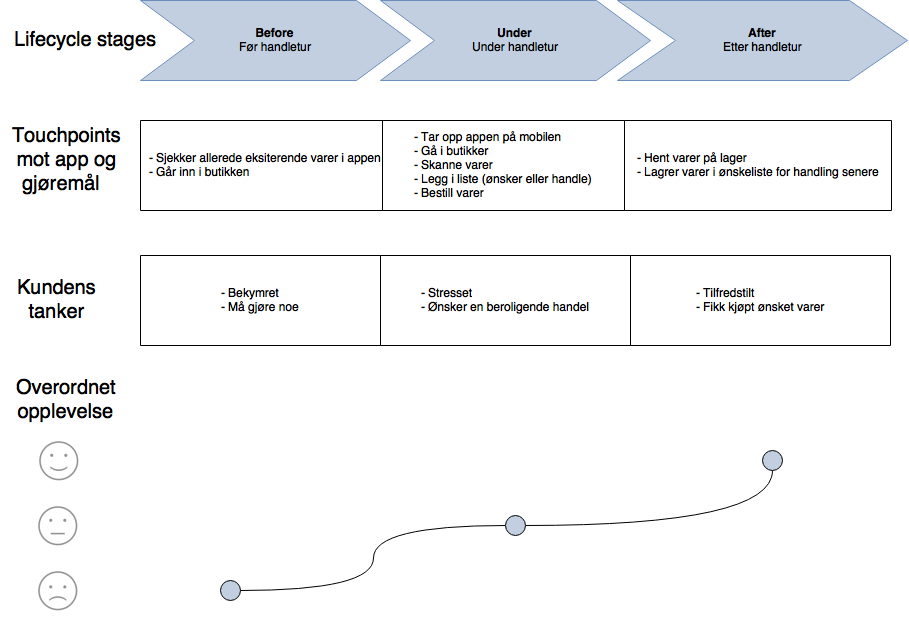
\includegraphics[scale=0.4]{images/customerjourneyBlueprint/cjKunde}
\centering %centering the image
\caption{Kundereise for kunde på Sirkus shopping}
\label{fig:customerKunde}
\end{figure}

\begin{figure}[H]
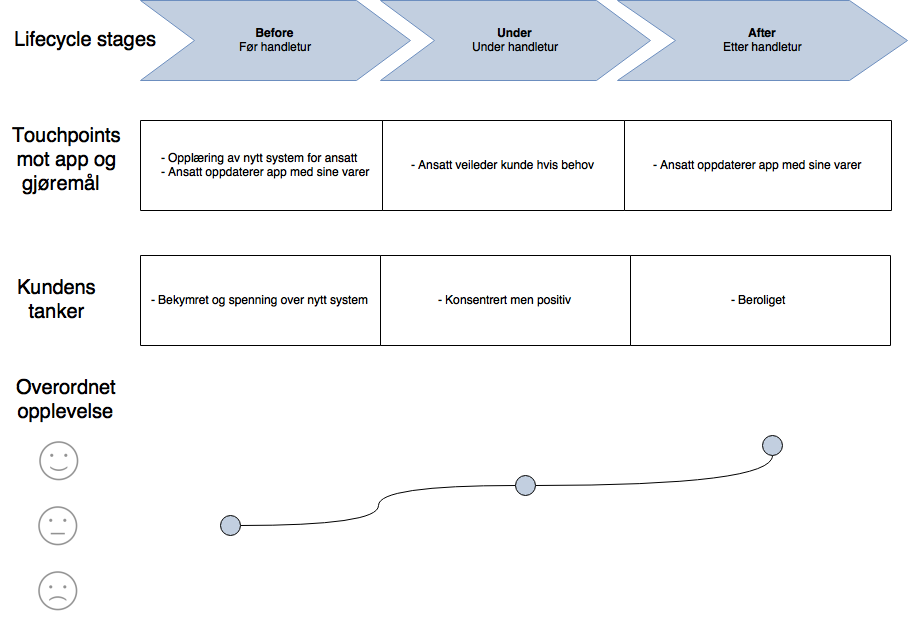
\includegraphics[scale=0.4]{images/customerjourneyBlueprint/cjAnsatt}
\centering %centering the image
\caption{Kundereise for ansatt i butikk på Sirkus shopping}
\label{fig:customerAnsatt}
\end{figure}

\begin{figure}[H]
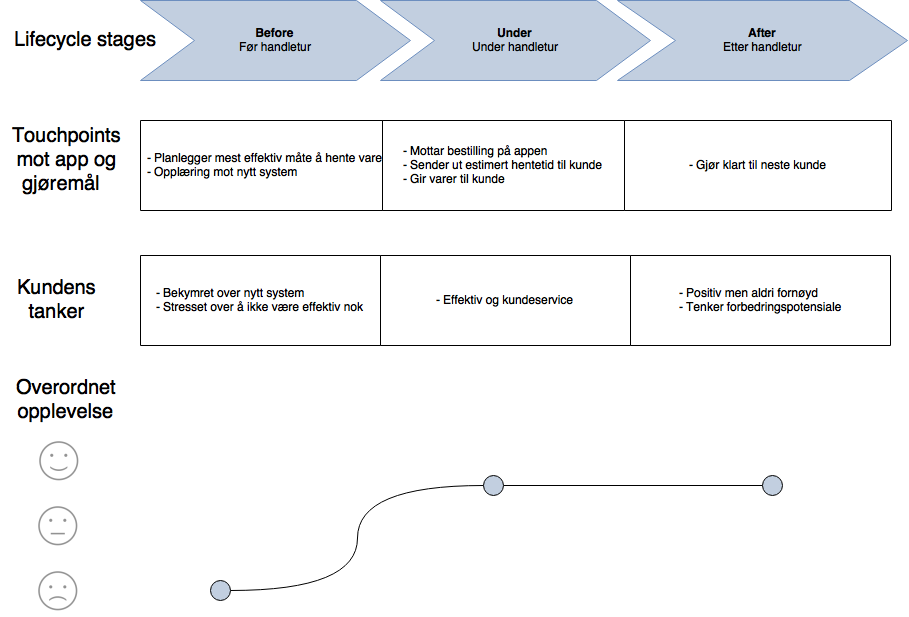
\includegraphics[scale=0.4]{images/customerjourneyBlueprint/cjLager}
\centering %centering the image
\caption{Kundereise for lagerarbeider på Sirkus shopping}
\label{fig:customerLager}
\end{figure}

\subsubsection{Blueprint}
\label{sec:blueprint}

Blueprint er en grafisk framvisning av alle aktiviteter som inngår i en tjeneste ved å følge alle personer og komponenter som er involvert og hvordan disse samarbeider for å gjennomføre en prosess\cite{servicedesign}.
Strukturen for et formelt blueprint-diagram er at den inneholder \textit{line of interaction} hvor kunde og media interagerer, \textit{line of visibility} hvor kunden ikke kan se hva som skjer i bakgrunnen og \textit{interaction} hvor business stopper og partnere stepper inn\cite{servicedesign}. I tillegg til dette er de 5p-ene som snakket om i Service Design 101 viktig i en blueprint\cite{servicedesign}. Under er disse presentert, med en berskrivelse av hvordan disse relaterer seg til vårt prosjekt i parentes fra Figur 5 Blueprint:
\begin{enumerate}
\item \textbf{People}, customers and employees encountered during the prosess.(Kunde, ansatt, lagerabeider)
\item \textbf{Place}, the physical space where the service is delivered.(Sirkus shopping)
\item \textbf{Props}, objects used to produce the service encounter.
\item \textbf{Partners}, other businesses that helps to produce the service. (Lagerarbeider, systemutviklere)
\item \textbf{Processes}, the workflows that are used to produce the service. (Effektiv handletur: opplæring blant alle tre aktører, utvikling av brukervennlig applikasjon, kontakt med bankterminal)
\end{enumerate} (SERVICE DESIGN 101: https://www.cooper.com/journal/2014/07/service-design-101)

\noindent På bakgrunn av kundereisene fra Kapittel \ref{sec:kundereise}: Kundereiser, lagde gruppen et felles blueprint-diagram, Figur \ref{fig:blueprint}, for disse kundene av applikasjonen. Grunnen til at vi laget en samlet blueprint var for å tydeliggjøre interaksjonen som skjer mellom kunden på Sirkus shopping, den ansatte, lagerarbeideren og applikasjonen selv. Dette førte til en bedre forståelse av hva som skjer onstage og backstage i bruk av applikasjonen før, under og etter en handletur på Sirkus shopping. 
\\\\
Symbol 1: Datamaskin = forespørsel til applikasjon\\
Symbol 2: Alfa = tilbakemelding fra applikasjon på forspørsel



%Denne bør kanskje legges sidelengs?
\begin{figure}[H]
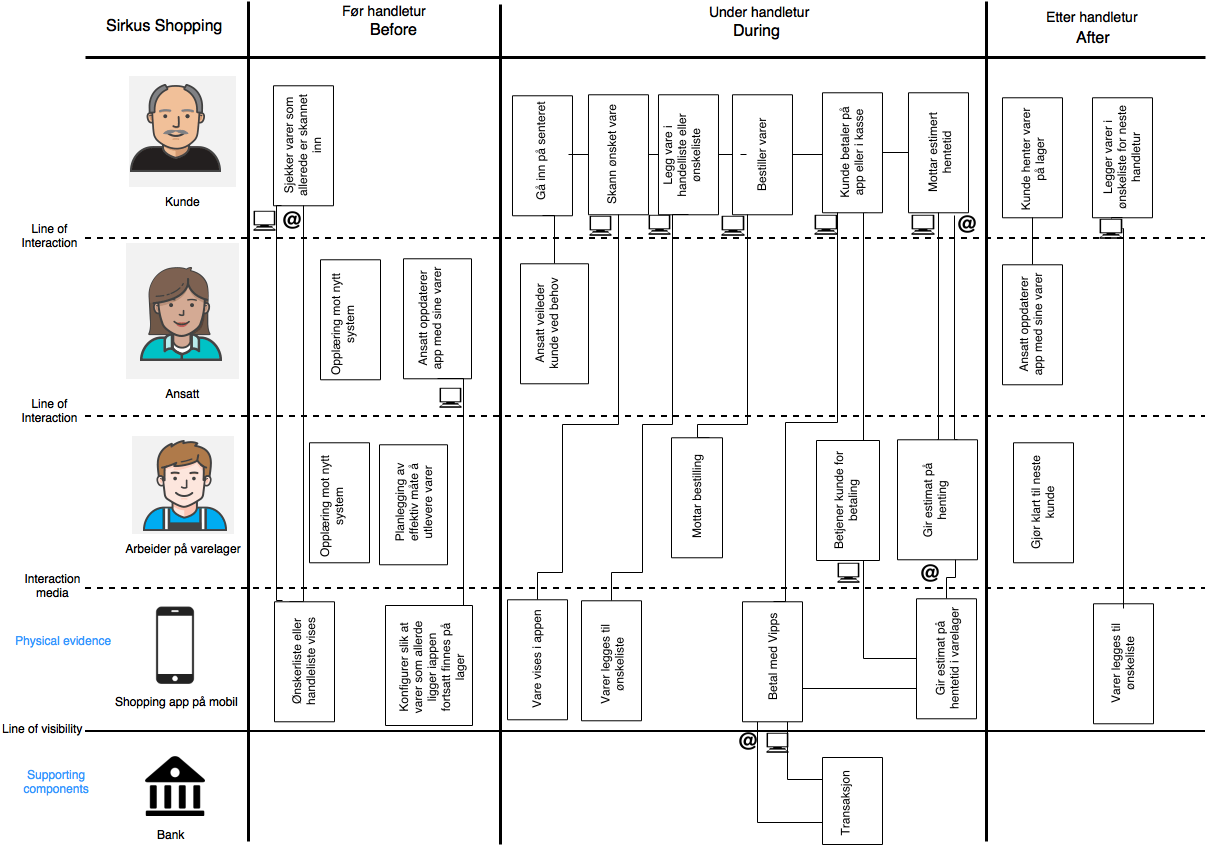
\includegraphics[scale=0.37]{images/customerjourneyBlueprint/blueprint5png}
\caption{Blueprint over handleprosess}
\label{fig:blueprint}
\end{figure}

\subsection{Funksjonelle krav}
På bakgrunn av ideen gruppen hadde bestemt seg for og analyseringen utført i de ulike tjenestedesign-aktivitetene, ble det utarbeidet en kravspesifikasjon før designet ble påbegynt. Dette ble gjort for å være sikker på at løsningene som ble valgt var gjennomtenkt og at appen ville ha best mulig funksjonalitet. Kravene er listet i Tabell \ref{tab:funksjonelle}.

\begin{table}[H]
    \caption{Funksjonelle krav}
    \label{tab:funksjonelle}
    \centering
    \begin{tabular}{|L{25em} L{18em}|}
    \hline
        \rowcolor[HTML]{D32F2F}
        \textbf{\textcolor{white}{Krav}} & \textbf{\textcolor{white}{Kommentar}}\\
        \rowcolor[HTML]{E6E6E6}
        Applikasjonen skal fungere på smarttelefoner & Gitt av oppgaveteksten\\
        Applikasjonen kan fungere på smartklokker & Gitt av oppgaveteksten
        \\
        \rowcolor[HTML]{E6E6E6}
        Brukeren må kunne logge inn. Da kan brukeren ha tilgang på handlelisten sin uansett enhet, og dersom man ikke har smarttelefon kan man låne en smarttelefon på senteret og logge inn på denne. Ved å logge inn kan brukeren også dele lister med andre brukere. & Logge inn via e-post. Logge inn via Facebook, gitt av oppgaveteksten. \\ 
        Brukeren må kunne opprette flere handlelister, slik at man kan sortere varene etter eget ønske. &\\
        \rowcolor[HTML]{E6E6E6}
        Brukeren må kunne slette handlelister. &\\
        Brukeren må kunne legge hele handlelister i handlekurven. &\\
        \rowcolor[HTML]{E6E6E6}
        Brukeren må kunne se totalpris på handlekurven i bunn av listen. &\\
        Brukeren må kunne endre handlekurven. &\\
        \rowcolor[HTML]{E6E6E6}
        Brukeren må kunne scanne et nytt produkt og legge det til i handlekurv eller liste. &\\
        Brukeren må kunne endre størrelse på produktene. &\\
        \rowcolor[HTML]{E6E6E6}
        Brukeren må kunne endre antall av produktene. &\\
        Brukeren må kunne navigere fram og tilbake mellom skjermene. &\\
         \rowcolor[HTML]{E6E6E6}
        Brukeren må kunne betale for handlekurven sin via appen. & Vipps eller tilsvarende\\
        Brukeren skal også kunne betale på senteret, får da beskjed om å henvende seg i skranken &\\
        \rowcolor[HTML]{E6E6E6}
        Brukeren må kunne vite hvor lenge det er til han eller hun kan hente varene. & \\
        Brukeren må kunne dele handlelisten med en venn. & E-post. Facebook.\\
        \rowcolor[HTML]{E6E6E6}
        Appen må være selvmotiverende, gitt i oppgaveteksten. & \\
        Appen må ha korrekt innhold & \\
        \hline
    \end{tabular}
\end{table}

\subsection{Ikke-funksjonelle krav}
Ikke-funksjonelle krav er vanskelig å måle. De handler ofte om ting som er svært subjektivt. De ikke-funksjonelle kravene i dette prosjektet er listet i Tabell \ref{tab:ikke-funksjonelle}, og det siste er f.eks. at appen må være visuelt tiltrekkende. Dette er svært vanskelig å vurdere, fordi det noe hver og en vurderer individuelt.

\begin{table}[H]
    \caption{Ikke-funksjonelle krav}
    \label{tab:ikke-funksjonelle}
    \centering
    \begin{tabular}{|L{25em} L{18em}|}
    \hline
        \rowcolor[HTML]{D32F2F}
        \textbf{\textcolor{white}{Krav}} & \textbf{\textcolor{white}{Kommentar}}\\
        \rowcolor[HTML]{E6E6E6}
        Appen må være oversiktlig & For at kunder skal forstå \\
        Appen må være intuitiv & For at kunder skal ønske å bruke appen\\
        \rowcolor[HTML]{E6E6E6}
        Appen må være brukbar & Gitt i oppgaveteksten\\
        Appen må være visuelt tiltrekkende & For at kunder skal vise andre og føle trang til å bruke\\
        \hline
    \end{tabular}
\end{table}
